\cleardoublepage
\chapter{Analysis}
\label{ch:analysis}
This chapter provides an overview of the research topic, and the tools and technologies used in this project.

\section{Research topic}\label{sec:research-topic}

The research topic of this project has pivoted over the course the project timeline.
Initially, the project was to create a C\# REST API connected to a machine learning module, capable of extracting desired information from images uploaded via the API.
A lot of focus was to be put into the API being well documented and hosted on Microsoft Azure.
It was also supposed to handle user authentication and logging of user statistics.
As the project went on, we shifted our focus from the API to the machine learning module.
This means the API will be more bare-bones, focused more on being able to

Our project is to create a solution that allows a user to take an image of a receipt, and automatically upload the
relevant data to a database.
This automates the process of handling travel receipts, thus making it less time-consuming and reduces the cost.
To achieve this, we will be using Optical Character Recognition software and machine learning\@.
The extracted data from the image consists of date, total amount, and the receipt type.

The app will consist of two main parts: The OCR, and the model that reads the data.
We are going to use a free open source OCR, named Tesseracts.
The OCR is what will allow us to extract text from the images.
This OCR will send all the text that is on the receipt in the form of an array to the model.
The model will then decide what information is the correct data to extract and keep.

With the app we also need to include an API that will talk with the app and talk with Simployers server.
This API gets the data from the model and will prompt the information that is selected for the user for a final
validation, before sending it to the Simployer database.
This will allow Simployer to easily search in the database based on the metadata that was extracted.

Another objective of this thesis is to analyse and compare solutions that already exists on the market.
And then create a prototype of each solution and connect them to the API\@.

\section{Tools}\label{sec:tools}
This section details the different tools that have been considered for use in the thesis.
\subsection{OCR engines}\label{subsec:ocr-engines}
There are many OCR engines that could be used for this thesis.
Three main ones have been selected for consideration.
These are Google Cloud Vision API, Amazon Textract, and Tesseract.
\subsubsection{Google Cloud Vision API}\label{subsubsec:API_Google}

Google Cloud Vision API contains a well optimised OCR and good variety of detection.
The detection features are listed in figure 2.1.

\begin{figure}[h]
    \center{\includegraphics[width=1\textwidth]{Images/googleAPI_features}}
    \caption{Overview of features (list from https://cloud.google.com/vision/pricing)}
    \label{fig:figure2.1}

\end{figure}

We can see that Google API offers everything from text recognition, to landmark location and crop Hints.
The Google API is know to be industry leading in the field, so this comes as no surprise.
This API will have almost everything you need to develop an application with text recognition.

The API also has a lot of features in their beta version which is not included in figure 2.1.
\clearpage

\begin{figure}[h]
    \center{\includegraphics[width=1\textwidth]{Images/googleAPI_prices}}
    \caption{Overview of prices (list from https://cloud.google.com/vision/pricing)}
    \label{fig:figure2.2}

\end{figure}

Google is the best in the field, but they are also the most expensive API to use.
The prices are calculated for every 1000th request
This means that you are getting the first 1000-requests free and then you will need to play 1.5\$ for each 1000-request you do on for example text detection.
If you have a request size of 50.000-requests this will be 49*1.5\$ = 73,5 dollars (620 NOK).
This will reset every month.

\subsubsection{Amazon Textract}\label{subsubsec:API_Amazon}

Amazon's AWS hosts a service called Textract.
This cloud-based service lets you upload an image to their text recognition software.

\textbf{Detect Document Text API}
This feature is the classic OCR feature that will extract text from a document.
Amazon will charge you 0.0015\$ per page (1.50\$ per 1000) for the first million pages, when you exceed 1 million the price wil go down to
0.0006\$ per page (0.6\$ per 1000)

\textbf{Table Extraction}
This is an improved version of Detect Document Text API. This will group the text in tables.
This is helpful with structured data, such as financial reports.
Amazon will charge you 0.015\$ per page (15.0\$ per 1000) for the first million pages, when you exceed 1 million the price wil go down to
0.01\$ per page (10\$ per 1000)

\textbf{Form Extraction}
This detects key-value pairs in documents, for example if your document has a field named "firstName" it will pair
it with "Mike".
This way "first name" would be the key and "Mike" would be the value.
This makes it easy to either sort it into a database or reuse the values in variables.
With normal OCR the relation is lost.
Amazon will charge you 0.05\$ per page (50\$ per 1000) for the first million pages, when you exceed 1 million the price wil go down to
0.04\$ per page (40\$ per 1000)

\textbf{Analyze Document API}

This is a combination of the tables and forms extraction
Amazon will charge you 0.065\$ per page (65\$ per 1000) for the first million pages, when you exceed 1 million the price wil go down to
0.05\$ per page (0.50\$ per 1000)

Note that Amazon changes their pricing on the region you are in (you might want to check the price for your region), they also do not include a free 1000 scans per a month.

\subsubsection{Tesseract}\label{subsubsec:Tesseract}
Tesseract is an open-source OCR engine that supports over 100 different languages.
It has the reputation of being one of the best open-source OCR engines.
It was created by HP in the 80's and later made open-source in 2005 and funded by google since 2006.
Most other OCR APIs today are build on top of this, like Google Cloud Vision API.

If this engine is used, code that takes advantage of the engine's built-in methods must be written.
When dealing with high-quality images and computer generated pdf receipts, writing code to extract the text is relatively simple.
When the images are of lower quality, more care must be given to pre-processing to improve the accuracy of the text
extraction.
This is because OCR software needs good contrast and little to no noise in the images.
Another problem is curved text, like in a book.
This might be the hardest ting to solve.

\section{Preprocessing}\label{sec:preprocessing}
Having images of ideal quality for use in an OCR is a luxury.
Images will often be of low quality or taken from suboptimal angles.
In order to mitigate the effects that low quality images will have on the text extraction accuracy, the images should go through a preprocessing stage before getting sent to the OCR software.

\subsection{Scaling the image}\label{subsec:scaling-the-image}
OCR software will have the best performance when given images between 300dpi and 600dpi.
Anything less will make it unreadable for the OCR and anything more will consume extra processing power with little to no improvement in accuracy.

\subsection{Skew correction}\label{subsec:skew-correction}
OCR engines use line segmentation to separate the text found in an image into different lines of data.
Therefore, it is important that the OCR is given images that are as straight as possible.
Skew correction is the part of the pre-processing pipeline that addresses this issue.

\subsection{Remove background noise}\label{subsec:remove-background-noise}
Image noise can reduce the accuracy of the OCR engine.
Because of this, removing noise in the background is very important to improve readability.
Applying a Gaussian blur is one way of reducing the noise in the image.

\subsection{Binarization}\label{subsec:how-to-create-contrast}
OCR engines are usually designed to handle input images with a black-and-white color scheme.
The process of converting a colorized or grayscale image to black-and-white is called binarization.
Once an image has gone through binarization, the background should be white and any foreground elements like text should be black.

If your image is in RGB format, it will first need to be converted to grayscale format before thresholding techniques can be used.
Adaptive thresholding is one such technique.
It involves partitioning the image into smaller regions, and calculating the threshold for what should be black and what should be white, in that region.

\section{Neural Networks}\label{sec:neural networks}
Artificial Neural Networks, or just Neural Networks as they are more commonly called, is a machine learning technique that learns by replicating the functions of the brain.
Our brain has billions of neurons connected through synapses in a massive network.
These neurons receive electrical signals from other neurons, and may send out their own electrical signal if their received signal was strong enough.
If the paths these signals take are used often, they will strengthen, allowing for a greater portion of electricity to be transfered.
This strengthening of pathways is how we as humans learn, and it is what we try to replicate with an Artifical Neural Network.
\begin{figure}[h]
    \center{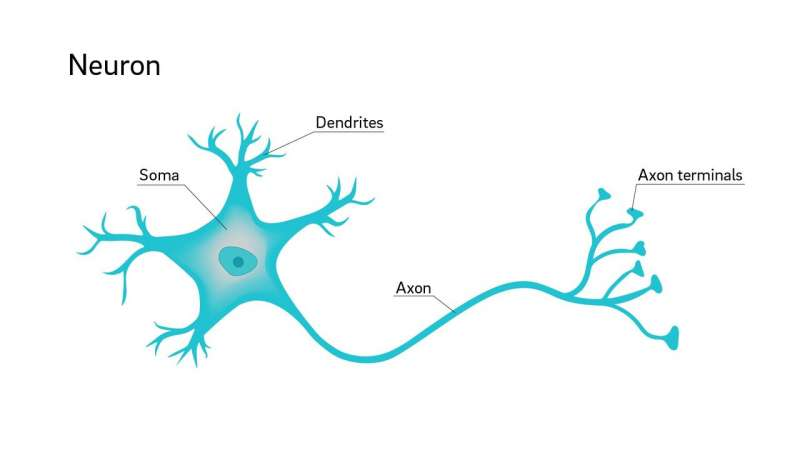
\includegraphics[width=1\textwidth]{Images/neuron}}
    \caption{Illustration of a neuron. https://scx1.b-cdn.net/csz/news/800a/2018/2-whyareneuron.jpg}
    \label{fig:figure2.3}
\end{figure}

The digital version of our neurons functions much in the same way.
They take inputs as numbers instead of electrical signals, and based on the strength of the connections the numbers arrived through, decide whether to fire off their own signal.
This process is illustrated in figure 2.4.
The input $x_n$ is the n-th signal being passed to the neuron.
The weight $w_n$ is the strength of the connection between the last neuron and this neuron.
All the inputs are multiplied with their corresponding weights, and summed up in the neuron, along with a bias for that neuron.
The activation function is what decides whether that neuron should fire of their signal to the next neuron or not.
In mathematical terms, the whole process looks like this: \[y = f(\left(\sum_{i=1}^{n} x_i w_i\right) + bias)\]
Adjusting the weights to make the neuron fire when it is supposed to it what makes the network learn.

\begin{figure}[h]
    \center{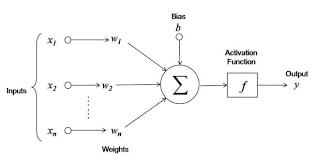
\includegraphics[width=1\textwidth]{Images/network_neuron}}
    \caption{Abstraction of a neuron for use in Artifical Neural Networks. https://encrypted-tbn0.gstatic.com/images?q=tbn:ANd9GcTRTFh3jYAWBE9gH0bKPJXykku4WDgqhJvQeQ&usqp=CAU}
    \label{fig:figure2.4}
\end{figure}

\section{Spacy}\label{sec:spacy}

Spacy is a program that gives context and relations to sentences and words.
With a foundation of machine learning.
This becomes a great tool for data extraction.
Spacy includes some great features that can make the production quick and easy.

\begin{figure}[h]
    \center{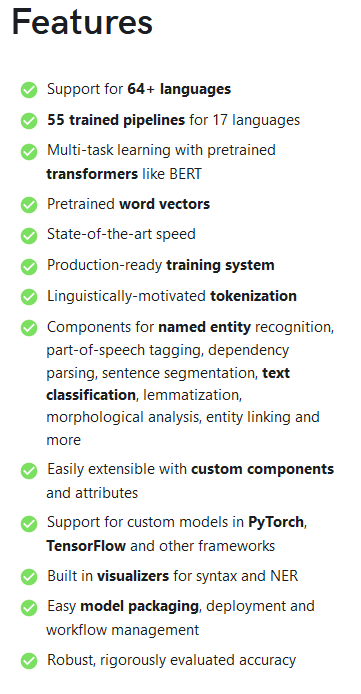
\includegraphics[width=0.5\textwidth]{Images/spacy-features}}
    \caption{Overview of spacy features. https://spacy.io/usage/spacy-101}
    \label{fig:figure2.5}
\end{figure}




\subsection{Arcitecture}\label{sec:architecture}


Spacy is structured around three main modules.
The language class, the vocab and Doc objects.
The language class is mainly focused on turning the data into doc objects.
Docs contains a sequence of tokens and their annotations and the vocab contains word vectors and lexical attributes.
With these spacy can centralize the strings and save memory(FOTNOTE: https://spacy.io/usage/spacy-101).
The product of these three central parts of the architecture and other sub classes will provide the architecture that is shown under. (KAN MAN POENGTERE TIL BILDER PÅ DENNE MÅTEN?)

\begin{figure}[h]
    \center{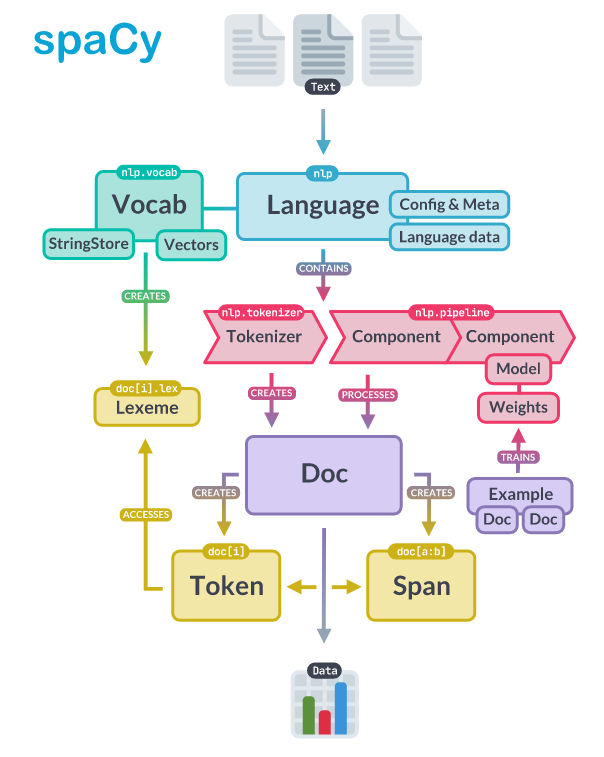
\includegraphics[width=0.5\textwidth]{Images/Spacy-architecture}}
    \caption{Overview of spacy architecture. https://spacy.io/usage/spacy-101}
    \label{fig:figure2.6}
\end{figure}

Spacy is filled with features, but we will focus on Named Entities.
Named entities is objects that is assigned a name.
Spacy does this by asking the model for a prediction.
However, the model is reliant on the data set it was trained on, this means that for a custom application.
Dedicated training could be necessary.
If we take a look at an example from their web page.
They got a simple string: Apple is looking at buying U.K. startup for \$1 billion
This will result with these labels. (https://spacy.io/usage/spacy-101)

\begin{figure}[h]
    \center{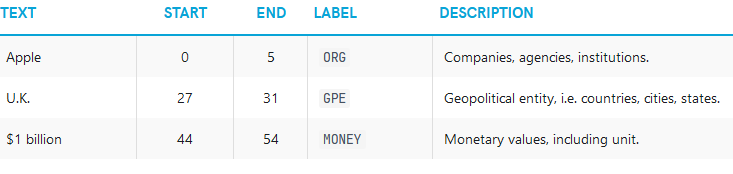
\includegraphics[width=0.5\textwidth]{Images/Spacy-ex}}
    \caption{Overview of spacy architecture. https://spacy.io/usage/spacy-101}
    \label{fig:figure2.6}
\end{figure}

As you can see, you will get labels that describes the words.
This combined with spacy's functionality to add relation to the words makes it easy to extract words or values you want.
When you got the label of the words, you can ask for a relation overview.
This will give you all the relations for your text.
Then you can write a simple script that loops through all the words and select the once labeled as ORG. Uou can then extract all the substrings that is labeled as money.
Then you would get out all the sentences that has and organisation talking about money in some form. 







